\documentclass{beamer}

\usepackage[utf8]{inputenc}
\usepackage[francais]{babel}
\setbeamerfont{caption}{size=\tiny}


\usetheme{Warsaw}

\title{%
  High-Res satellite imagery for human density prediciton\\
  \large \\
    }

\author{\textsc{Youcef} - \textsc{Kacer}}
\date{22 Novembre 2016}

\begin{document}
\begin{frame}
Data Science Project
\end{frame}
\section{Summary}
\begin{frame}
\frametitle{Summary}
%\begin{description}
%\item[-] Presentation
%\item[-] Data source and checking
%\iten[-] Feature extraction
%\item[-] Regression
%\item[-] Classification
%\end{description}
\end{frame}

\section{Presentation}

\begin{frame}
- Population census expensive using conventional methods\\
- How High-resolution satellites images could explain human density?\\
- How to transform HR satellite images to explain human density?\\
\end{frame}

\section{Landsat-8 satellite imagery}
\subsection{Covering}

\begin{frame}
Total earth covering defined by path,row grid pattern and achieved every 16 days
\begin{figure}
  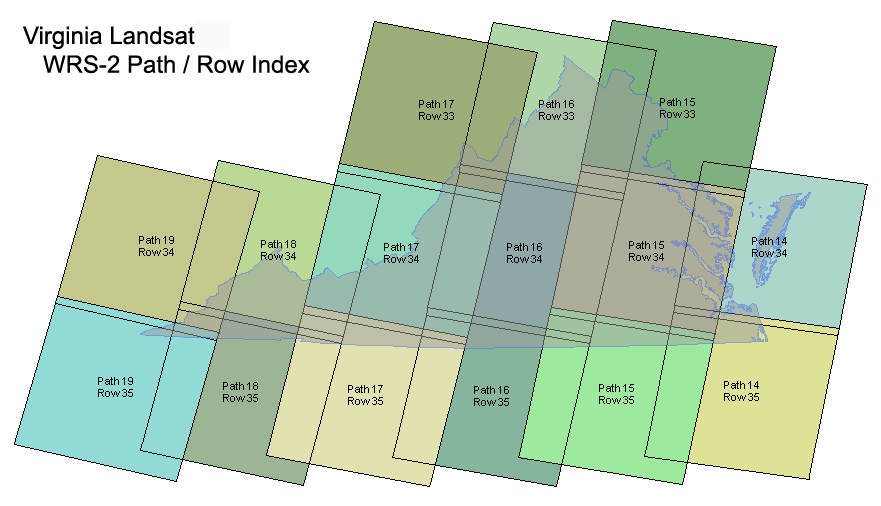
\includegraphics[scale=0.13]{images/covering/wrs.png}
  \caption{Landsat-8 grid covering (path,row) for Virginia ($USA$) }
\end{figure}
\end{frame}

\subsection{Georeferencing}

\begin{frame}
Landsat-8 images are georeferenced : each pixel has (x,y) coordinates in a certain Projection Coordinates 
System (\begin{itshape}UTM Mercator\end{itshape})\\
\begin{minipage}{.5\textwidth}
\begin{figure}
  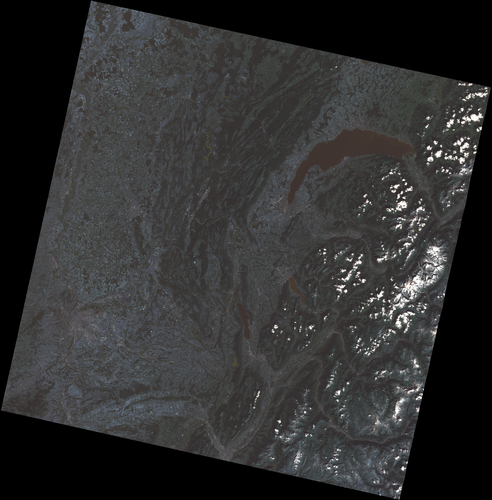
\includegraphics[scale=0.2]{images/georeferencing/Thonon_landsat.png}
  \caption{Landsat-8 grid covering (path,row) for Virginia ($USA$) }
\end{figure}
\end{minipage}
\begin{minipage}{.5\textwidth}
 upper left point : (,)
 upper right point : (,)
 bottom right point : (,)
 bottom left point : (,)
\end{minipage}



\end{frame}

\begin{frame}
Landast-8 georeferencing can be checked comparing with another georeferenced source like $IGN$ using a $SIG$ (open source $QGIS$).\\
\centering
\begin{minipage}{.5\textwidth}
    \centering
    \begin{figure}
        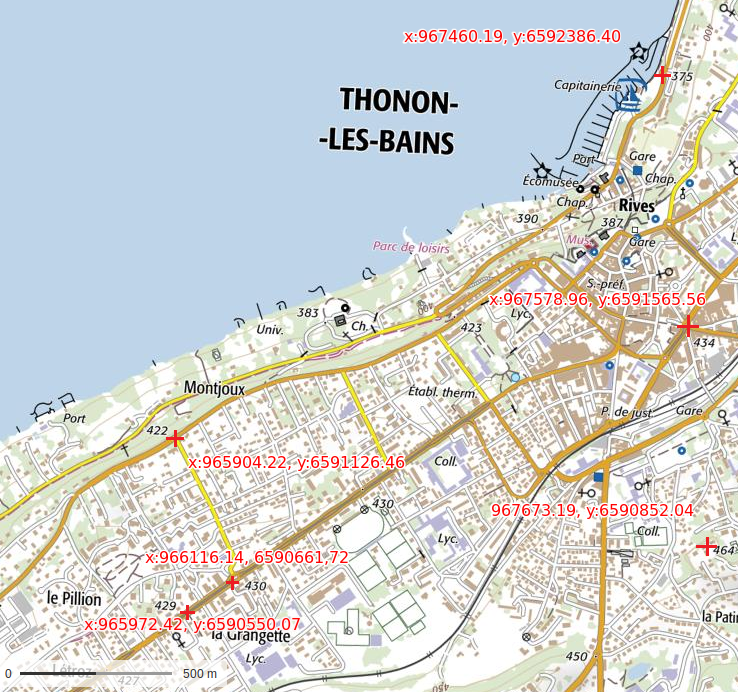
\includegraphics[scale=0.13]{images/georeferencing/ign-points-Thonon.png}
        \caption{IGN georeferenced image from $Lambert$ $93$ }
    \end{figure}
\end{minipage}%
\begin{minipage}{.5\textwidth}
    \centering
    \begin{figure}
        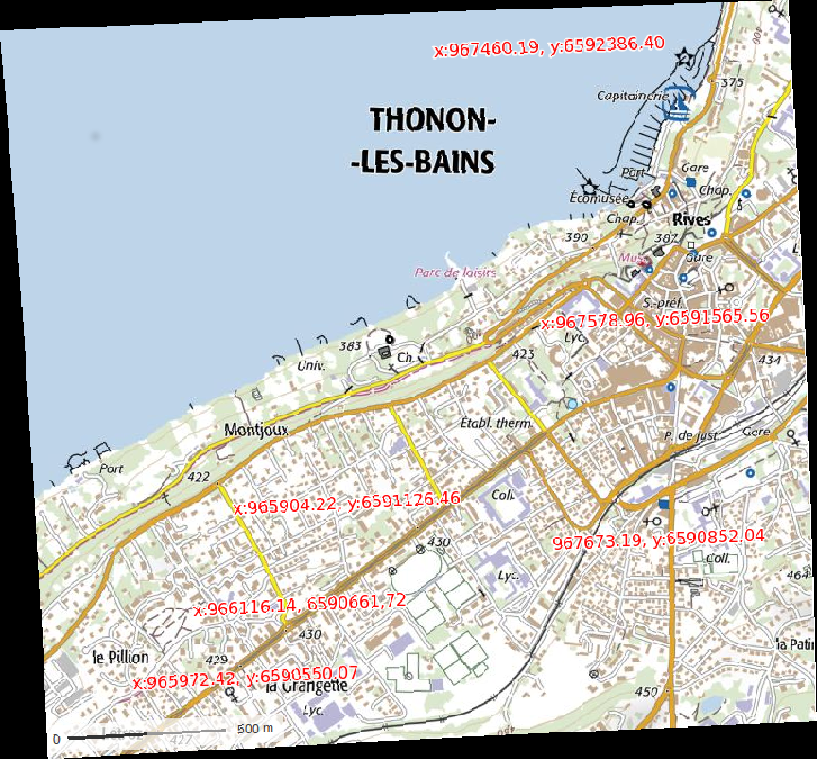
\includegraphics[scale=0.09]{images/georeferencing/qgis-resultat.png}
        \caption{IGN georeferenced image to $UTM$ $Mercator$}
    \end{figure}
\end{minipage}

    \centering
    \begin{figure}
        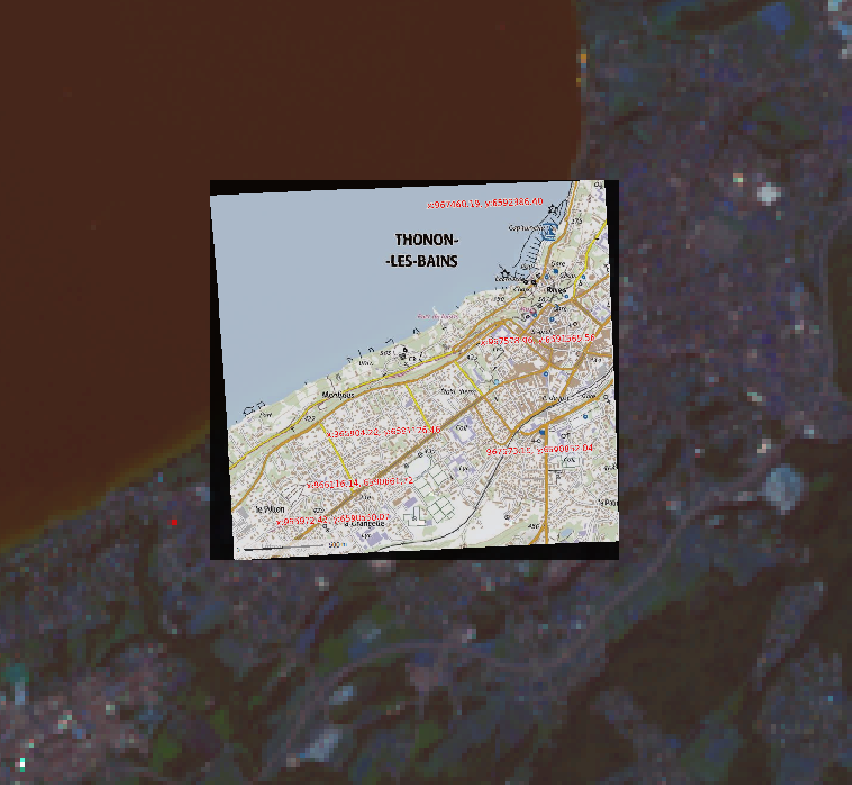
\includegraphics[scale=0.09]{images/georeferencing/qgis-superposition0.png}
        \caption{IGN georeferenced image ($UTM$ $Mercator$) superposed with Landsat-8 georeferenced image ($UTM$ $Mercator$) }
    \end{figure}

\end{frame}

\end{document}